\section{Assessment of Pain}
Pain is described as a complex and subjective experience that poses a number of measurement challenges due to its subjective nature. Nevertheless, pain measurements are necessary for pain studies as well as the evaluation of methods to control pain.~\cite{Jensen2001} There is no valid and reliable method of objectively quantifying pain at the moment. However, despite the challenges that pain measurement present, several tools and approaches can be employed in order to collect useful pain estimates.~\cite{Younger2010} The aim of pain assessment is to diagnose the cause, understand the impact, identify appropriate pain relief strategies and evaluate their effectiveness~\cite{Briggs2010}.

There are different dimensions of pain experience that can be assessed: pain intensity, pain affect, pain quality and pain location. Pain intensity defined as how much the pain hurts, where pain affect is more complex. Pain affect refers the degree of emotional arousal or changes in action due to the sensory experience of pain. The quality of pain is about the physiological sensations associated with pain. 

\subsection{Assessment of Acute Pain}
Pain assessment of acute pain include history of pain and evaluation of regarding the different aspects of pain including functional impairment~\cite{Gupta2014}. The intensity of pain can be assess using unidimensional scales, which explore only one dimension of pain~\cite{Jensen2001}. % Changes in pain intensity should only be compared individually and not between subjects, as pain is a subjective experience.

\subsubsection{Unidimensional scales}
One commonly used unidimensional tool is the Verbal Rating Scales (VRS) which consists of a list of adjectives describing different levels of pain intensity, as illustrated on \figref{fig:VRS}. This type of scales are easy to administer, score and apprehend. However, it has several statistical disadvantages and criticism raised due to the fact that assumes equal intervals between adjective.~\cite{Jensen2001} For this particular reasons along with others it is used when the patient's conditions require it~\cite{Jensen1986}. 

\begin{figure}[H]
	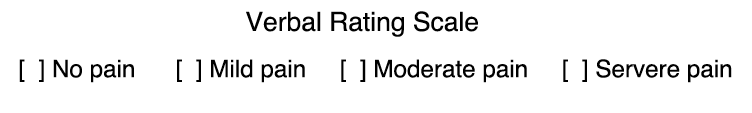
\includegraphics[width=0.5\textwidth]{figures/VRS.png} 
	\caption{Verbal Rating Scales (VRS). Modified~\cite{Jensen2001}}
	\label{fig:VRS}  
\end{figure}   

Other possibility of unidimensional scales is a visual analogue scale (VAS). VAS consists of a 10 cm line, as shown in \figref{fig:VAS},the ends of this line are labeled as the extremes of pain. The scale is scored by measuring the distance from 'no pain' end to the patient's mark. This fact makes the VAS more sensitive to changes in pain intensity. However, one of the drawbacks is that scoring time is higher than for other methods.~\cite{Jensen2001} 

\begin{figure}[H]
	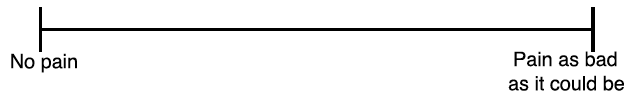
\includegraphics[width=0.5\textwidth]{figures/VAS.png} 
	\caption{Visual analogue scale (VAS). Modified~\cite{Jensen2001}}
	\label{fig:VAS}  
\end{figure}   

Numerical Rating Scale (NRS), which is illustrated on \figref{fig:NRS}, is also within unidimensional tools of pain intensity measure. NRS consits of an numerical scale from 0 to 10, being described 0 as 'no pain' and  10 equal to 'higest level of pain'. The advantage of NRS is that it not requires patients mobility because the response is given verbally. NRS is a valid method and demonstrate positive and significant correlations with other measures of pain intensity \cite{Jensen2001}. 

\begin{figure}[H]
	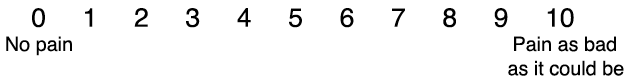
\includegraphics[width=0.5\textwidth]{figures/NRS.png} 
	\caption{Numerical Rating Scale (NRS). Modified~\cite{Jensen2001}}
	\label{fig:NRS}  
\end{figure}   

Another method is to use pictures or face scales to illustrate facial expressions of different intensities of pain. Even though the primary purpose of this scales were to offer individuals with written language or cognitive difficulties an option to express pain intensity, there is evidence that they are valid methods \cite{Jensen2001}. 

\subsection{Assessment of Chronic Pain}
Chronic pain is complex to assess as the pain affect their functions, quality of life, emotional state, vocational status, social life and well-being, why multidimensional scales are necessary~\cite{Ebert2010}. Therefore the assessment of pain beside multidimensional scales should include physiological assessment.

\subsubsection{Multidimensional scales}
Multidimensional scales\fxnote{Be aware that there are many different questionnaires designed for general pain, different aspects of pain, or various pain conditions.} are convenient in relentless pain conditions. Multidimensional scales measure several dimensions of pain with different combinations of these dimensions. These scales offer a more detailed reflection of the patient's pain experience \cite{Briggs2010}. 

There are six commend used measurement in clinical trials for assessing pain quality. Three of them are editions of McGill Pain Questionnaire (MPQ) and two of them within the field of neuropathic pain and the last one is the Pain Quality Assessment Scale(PQAS).For estimating the location of pain is pain drawing often used, which involve a front and back drawing of the human body. A second commend used methods is the checklist, which is a simple list of possible site of pain.~\cite{Jensen2001} 

The most commend used is MPQ, which consists of 78 words and describe the pain in sensory, affective and evaluative terms. These tems are arranged in groups acoording to the quality of pain and intensity of this pain. A 6-point VRS is used to determ the intensity of the pain. The MPQ is proved as a valid method support by several studies. One disadvantage of the MPQ is the length and complexity, why a brief form of this questionnaire has been introduced, the short-form McGill Pain Questionnaire (SF-MPQ)~\cite{Katz2001}. \fxnote{15 different descriptors in sensory and affective terms. Each descriptor is rated on a 4-point VRS scale.}

Another scale, breif pain inventory (BPI), was developed to assess cancer pain and have been proven as a useful instrument to asses different kinds of pain in several clinical settings. The BPI measures pain severity, pain quality and the disturbance caused in the patients daily life. Two subscale scores pain intensity and pain interference~\cite{Katz2001}.  

\subsubsection{Physiological assessment}
The most commend used for physiological assessment is Back Depression Inventory (BDI), which is used for patients with depression associated to their chronic pain. BDI consist of a questionnaire of 21 question related to the depression. The score of BDI indicated the if the depression is minor, moderate or server. The Spielberger-State-Trait Anxiety Inventory is often used for patient with anxiety beside the chronic pain and consist of 40 item that assess both the stare and trait anxiety.  Furthermore, is the Minnesota Multiphasic Personality Inventory and Coping Strategies Questionnaire. 

%\subsection{Psychological Methods}
%Quantitative sensory testing (QST) evaluates the integrity of the entire sensory neuraxis receptor to the cortex. Even though QST has recieved criticism for being subjective, it is a reliable test. Brain imaging studies provided evidence that subjective pain magnitude scores are associated with objectively measured neural activity in areas of the brain involved in pain processing. QST include different modalities of stimulation, such as thermal, mechanical, electrical, ischemic and chemical. This method provide two different assessments of pain. On the one hand the  evaluation of endogenous pain, which is the pain that the patient experiences due to the disease process. On the other hand, the assessment of induced pain, in order to experiment on pain mechanisms or therapy. \cite{Yarnitsky2006}


\section{Assessment of Experimental Pain}
As a result to a set of experimental noxious stimuli, it is possible to obtain different parameters such as, pain thresholds, tolerance or suprathreshold pain intensities. Threshold is defined as the stimulus that produces an arbitrary, but defined, level of performance. There is a distinction between receptor or absolute threshold and psychophysical or sensory threshold. Absolute threshold is the energy required to elicit response in the primary afferent while the psychophysical or sensory threshold, is the minimal energy necessary to reach perception. Due to the fact that receptor threshold is lower than sensory threshold, the sensory threshold is a convenient parameter which offers the transition point between non-painful and painful stimulus. \cite{Yarnitsky2006}


\subsubsection{Types of physiophysical methods}
Psychophysical research has been mostly concentrated on thresholds measurement owing to, the desire to isolate low-level sensory mechanisms using operationally defined tasks that are intended to minimize the roles of perception and cognition \cite{Pelli2010}. The three most commend methods used for testing the perception in stimulus detection is the methods of adjustment, methods of limits and methods of constant stimuli.

\textbf{Methods of adjustment}: The magnitude of a stimulus dimension is adjusted, until a prespecified criterion is reached. This method is useful for obtaining a rough threshold estimate to guide the choice of stimulus magnitudes for a forced-choice procedure, when there are different conditions to be measured. \cite{Kingdom2016}

\textbf{Methods of limits}: The magnitude of the stimulus are presented in eater a ascending or a descending order.
The subject indicates whether or not the stimulus differs from the baseline. Accordingly, the threshold in each case is the stimulus magnitude at which the response switches from non perception to perception and/or vice versa. \cite{Kingdom2016}\fxnote{Look at the uncomment part. I am not sure if it relevant. I think it nice to know but needed}
%One of the drawbacks of this method is that the observer may get used to reporting that is perceiving a stimulus or not. As a result, he or she continues to give the same response even at stimulus magnitudes that are higher or lower than the threshold. This phenomena is the error of habituation. Contrarily, the observer may anticipate the response and make a premature judgment, which is call the error of expectation. Another disadvantages using this method is that the parameter value from perception to non-perception differ from non-perception to perception value, due to different artifacts \cite{Hock2010}.

\textbf{Method of constant stimuli}: The magnitude of the stimuli is randomly selected from a predefined set. This range is selected to straddle the threshold value. This method generates data, when this data fitted with the appropriate psychometric function, provides the most accurate estimates of the threshold. The choice of this stimulus set sometimes demand pilot work to obtain an estimate of the threshold. 




